\documentclass{article}
\usepackage{blindtext}
\usepackage[a4paper, bottom=1in, top=1in, right=0.75in, left=0.75in]{geometry}
\usepackage{fancyhdr}
\usepackage{minted}
\usepackage[most]{tcolorbox}
\usepackage{graphicx}
\definecolor{mygray}{rgb}{0.8,0.8,0.8}

\lstset{%
    basicstyle=\ttfamily,
    breaklines = true,
    backgroundcolor=\color{mygray},
}

\usepackage{realboxes}
\usetikzlibrary{chains,shadows.blur}
\usemintedstyle{lovelace}

\definecolor{lightgray}{rgb}{0.74, 0.74, 0.74}

\DeclareDocumentCommand{\clist}{v}{%
    \Colorbox{mygray}{\csname lstinline\endcsname!#1!}%
}

\begin{document}

\rhead{\thepage}

% \rfoot{\thepage}

\lhead{CS215 - Theory of Computation - Marek Chrobak}

\pagestyle{fancy}

\cfoot{}

% title
\begin{center}

\large{\textbf{CS215 ASSIGNMENT 2}}

Due Wednesday, February 7, 11:59PM

Ivan Neto

\end{center}

\vskip 0.2in

\noindent\textbf{Problem 1:} (i) Apply available expression analysis to the following
CFG to find the AvailIn set for each BB ; (ii) Based on the results of available
expression analysis, use GCSE (Global Common Subexpression Elimination) to find out
the redundant computations and remove them.

\newcolumntype{M}[1]{>{\centering\arraybackslash}m{#1}}
\newcolumntype{N}{@{}m{0pt}@{}}

\begin{center}
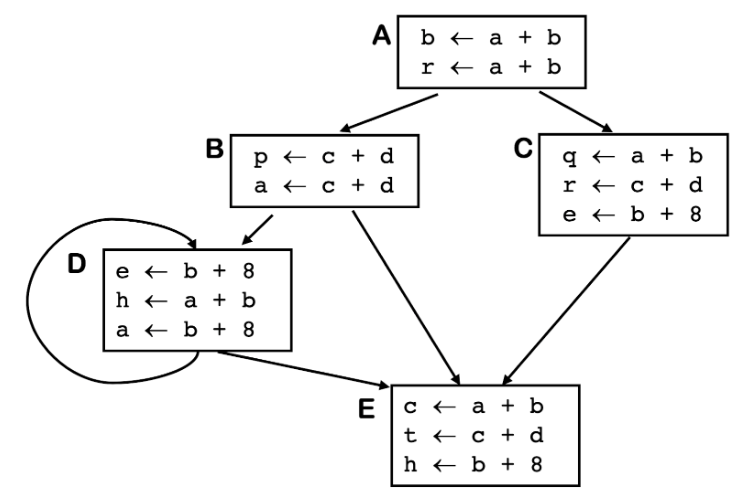
\includegraphics[scale=0.5]{prob1.png}
\end{center}

\noindent
{\renewcommand{\arraystretch}{2}
\begin{tabularx}{\textwidth}{|X|X|X|X|X|X|}
\hline
Block & A & B & C & D & E \\
\hline
Block & A & B & C & D & E \\ [1em]
\hline
\end{tabularx}
}

\vskip 0.1in

\noindent \textit{Tips: to apply GCSE, you can first find the redundant computations
(expressions), then create the global hash names only for those expressions,
and finally, transform the CFG to remove the redundancies.}


\vskip 0.2in

\noindent \textbf{Solution:}

\vskip 0.1in

\noindent \textbf{Solution 1.1)} Adding version numbers

\vskip 0.2in

% \newcommand*{\yellowemph}[1]{%
% \tikz[baseline]\node[rectangle, fill=green, inner sep=0mm,anchor=base]{#1};%
% }

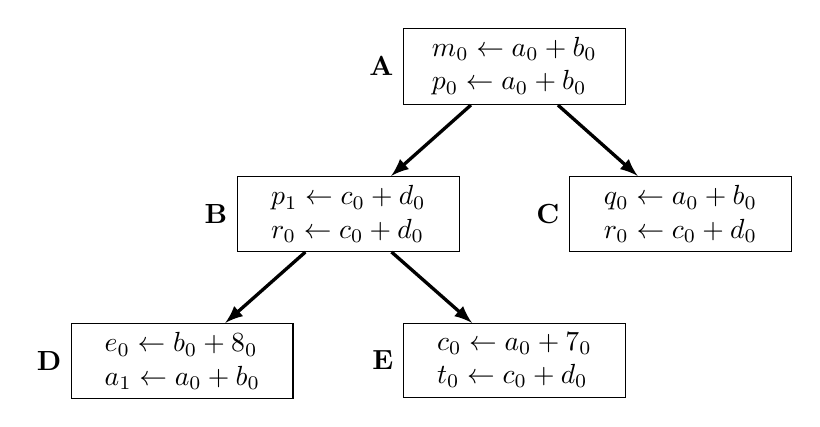
\begin{tikzpicture}[
    node distance = 9mm and 14mm,
    nodestyle/.style = {draw,
                        minimum width=8em,
                        minimum height=2em,
                        align=left,
                        font=\ttfamily},
    arr/.style       = {very thick,
                       -latex}
]
\node (q0) [nodestyle, label=left:\textbf{A}] {
$m_0 \leftarrow a_0 + b_0$ \\
$p_0 \leftarrow a_0 + b_0$
};
\node (q1) [nodestyle, below=of q0, xshift=-6em, label=left:\textbf{B}]    {
$p_1 \leftarrow c_0 + d_0$ \\
$r_0 \leftarrow c_0 + d_0$
};
\node (q2) [nodestyle,below=of q0, xshift=6em, label=left:\textbf{C}] {
$q_0 \leftarrow a_0 + b_0$ \\
$r_0 \leftarrow c_0 + d_0$
};
\draw[arr] (q0) -- (q1);
\draw[arr] (q0) -- (q2);
\node (q3) [nodestyle,below=of q1, xshift=-6em, label=left:\textbf{D}] {
$e_0 \leftarrow b_0 + 8_0$ \\
$a_1 \leftarrow a_0 + b_0$
};
\node (q4) [nodestyle,below=of q1, xshift=6em, label=left:\textbf{E}] {
$c_0 \leftarrow a_0 + 7_0$ \\
$t_0 \leftarrow c_0 + d_0$
};
\draw[arr] (q1) -- (q3);
\draw[arr] (q1) -- (q4);
\end{tikzpicture}

\vskip 0.3in

\noindent \textbf{Solution 1.2)} Adding a hash table status next to each basic block. Also applying Value Numbering.

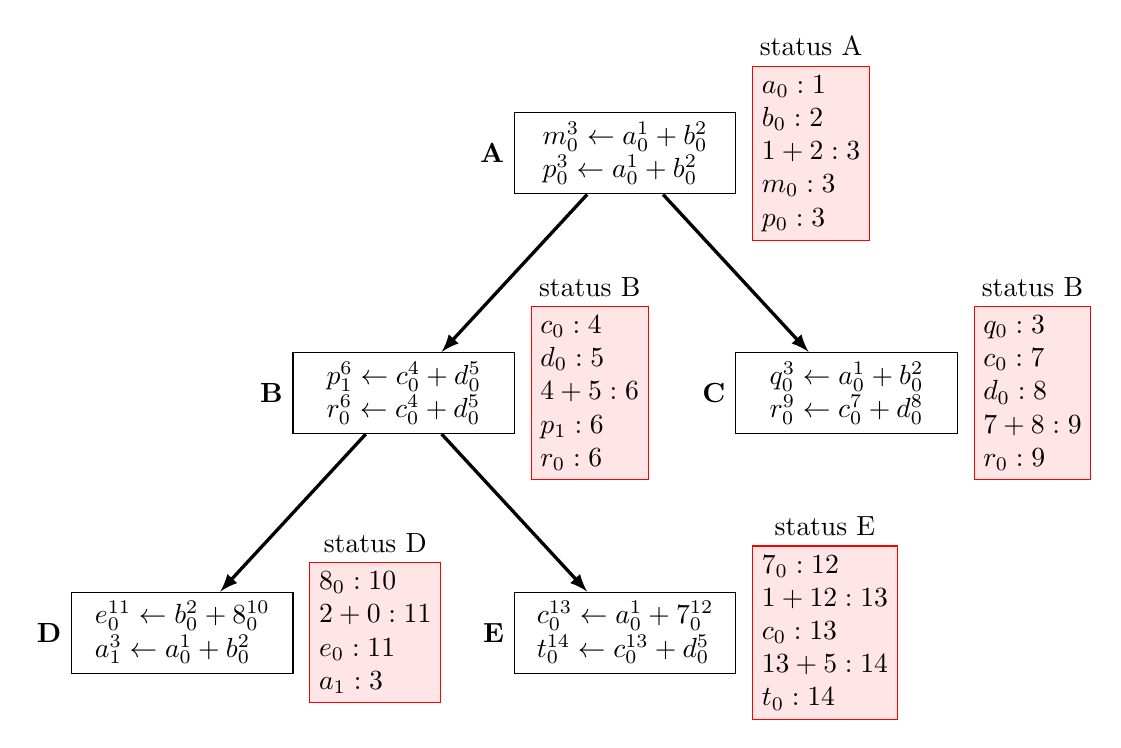
\begin{tikzpicture}[
    node distance = 20mm and 2mm,
    nodestyle/.style = {draw,
                        minimum width=8em,
                        minimum height=2em,
                        align=left,
                        font=\ttfamily},
    hashstyle/.style = {draw=red,
                        fill=red!10,
                        minimum width=4em,
                        minimum height=2em,
                        align=left,
                        font=\ttfamily
                        },
    arr/.style       = {very thick,
                       -latex}
]
\node (q0) [nodestyle, label=left:\textbf{A}] {
$m_0^{3} \leftarrow a_0^{1} + b_0^{2}$ \\
$p_0^{3} \leftarrow a_0^{1} + b_0^{2}$
};

\node (q1) [nodestyle, below=of q0, xshift=-8em, label=left:\textbf{B}]    {
$p_1^{6} \leftarrow c_0^{4} + d_0^{5}$ \\
$r_0^{6} \leftarrow c_0^{4} + d_0^{5}$
};

\node (q2) [nodestyle,below=of q0, xshift=8em, label=left:\textbf{C}] {
$q_0^{3} \leftarrow a_0^{1} + b_0^{2}$ \\
$r_0^{9} \leftarrow c_0^{7} + d_0^{8}$
};

\node (q3) [nodestyle,below=of q1, xshift=-8em, label=left:\textbf{D}] {
$e_0^{11} \leftarrow b_0^{2} + 8_0^{10}$ \\
$a_1^{3} \leftarrow a_0^{1} + b_0^{2}$
};

\node (q4) [nodestyle,below=of q1, xshift=8em, label=left:\textbf{E}] {
$c_0^{13} \leftarrow a_0^{1} + 7_0^{12}$ \\
$t_0^{14} \leftarrow c_0^{13} + d_0^{5}$
};

\draw[arr] (q0) -- (q1);
\draw[arr] (q0) -- (q2);
\draw[arr] (q1) -- (q3);
\draw[arr] (q1) -- (q4);

\node (h0) [hashstyle, label=above:status A, right=of q0] {
    $a_0: 1$ \\
    $b_0: 2$ \\
    $1+2: 3$ \\
    $m_0: 3$ \\
    $p_0: 3$
};
\node (h1) [hashstyle, label=above:status B, right=of q1] {
    $c_0: 4$ \\
    $d_0: 5$ \\
    $4+5: 6$ \\
    $p_1: 6$ \\
    $r_0: 6$
};
\node (h2) [hashstyle, label=above:status B, right=of q2] {
    $q_0: 3$ \\
    $c_0: 7$ \\
    $d_0: 8$ \\
    $7+8: 9$ \\
    $r_0: 9$
};
\node (h3) [hashstyle, label=above:status D, right=of q3] {
    $8_0: 10$ \\
    $2+0: 11$ \\
    $e_0: 11$ \\
    $a_1: 3$
};
\node (h4) [hashstyle, label=above:status E, right=of q4] {
    $7_0: 12$ \\
    $1+12: 13$ \\
    $c_0: 13$ \\
    $13+5: 14$ \\
    $t_0: 14$
};

\end{tikzpicture}

\vskip 0.3in

\noindent \textbf{Solution 1.3)} Writing down transformed EBB after removing redundancies

\vskip 0.2in

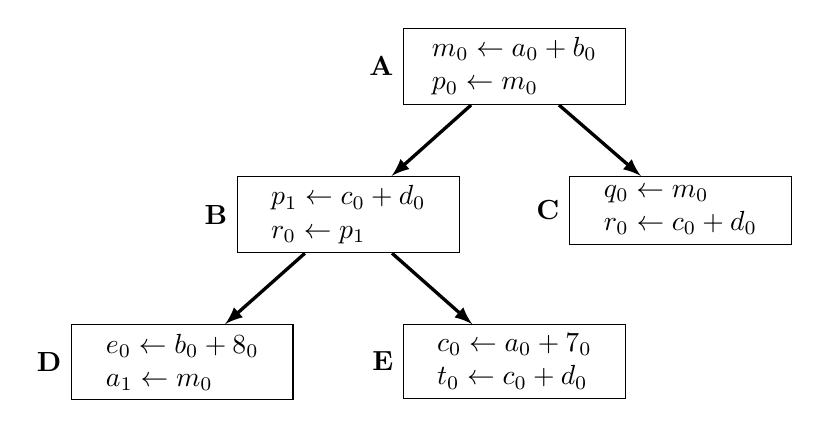
\begin{tikzpicture} [
    node distance = 9mm and 14mm,
    nodestyle/.style = {draw,
                        minimum width=8em,
                        minimum height=2em,
                        align=left,
                        font=\ttfamily},
    arr/.style       = {very thick,
                       -latex}
]
\node (q0) [nodestyle, label=left:\textbf{A}] {
$m_0 \leftarrow a_0 + b_0$ \\
$p_0 \leftarrow m_0$
};
\node (q1) [nodestyle, below=of q0, xshift=-6em, label=left:\textbf{B}]    {
$p_1 \leftarrow c_0 + d_0$ \\
$r_0 \leftarrow p_1$
};
\node (q2) [nodestyle,below=of q0, xshift=6em, label=left:\textbf{C}] {
$q_0 \leftarrow m_0$ \\
$r_0 \leftarrow c_0 + d_0$
};
\draw[arr] (q0) -- (q1);
\draw[arr] (q0) -- (q2);
\node (q3) [nodestyle,below=of q1, xshift=-6em, label=left:\textbf{D}] {
$e_0 \leftarrow b_0 + 8_0$ \\
$a_1 \leftarrow m_0$
};
\node (q4) [nodestyle,below=of q1, xshift=6em, label=left:\textbf{E}] {
$c_0 \leftarrow a_0 + 7_0$ \\
$t_0 \leftarrow c_0 + d_0$
};
\draw[arr] (q1) -- (q3);
\draw[arr] (q1) -- (q4);
\end{tikzpicture} 

\newpage


\noindent \textbf{Problem 2:} Consider the following control flow graph (CFG) and answer the following questions.


\begin{itemize}
    \item[1.] Find all the EBBs in the CFG;
    \item[2.] Check if any of the following block sets (and their associated edges) may form a region:
    \begin{itemize}
        \item[a)] $\{B, C, D\}$
        \item[b)] $\{B, C, D, E\}$ 
        \item[c)] $\{C, D, E, F\}$
        \item[d)] $\{B, C, D, E, F, G\}$ 
    \end{itemize} 
    \item[3.] Find the dominator set for each basic block;
    \item[4.] Build the dominance tree for the CFG;   
\end{itemize}

\vskip 0.3in

\begin{center}
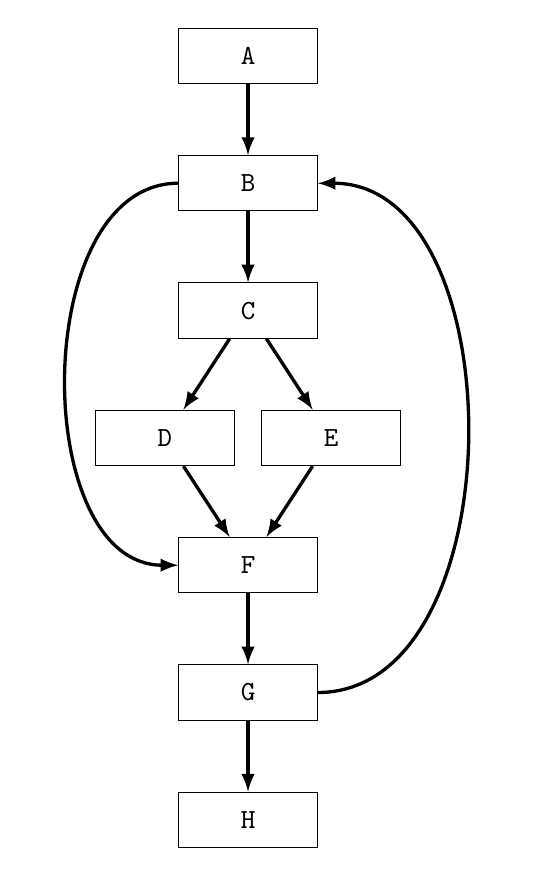
\begin{tikzpicture}
[
    node distance = 9mm and 14mm,
    nodestyle/.style = {draw,
                        minimum width=5em,
                        minimum height=2em,
                        font=\ttfamily},
    arr/.style       = {very thick,
                       -latex}
]

\node (q0) [nodestyle] {
\textbf{A}
};
\node (q1) [nodestyle, below=of q0] {
\textbf{B}
};

\draw[arr] (q0) -- (q1);

\node (q2) [nodestyle, below=of q1] {
\textbf{C}
};

\draw[arr] (q1) -- (q2);

\node (q3) [nodestyle, below=of q2, xshift=-3em] {
\textbf{D}
};

\node (q4) [nodestyle, below=of q2, xshift=3em] {
\textbf{E}
};

\draw[arr] (q2) -- (q3);
\draw[arr] (q2) -- (q4);

\node (q5) [nodestyle, below=of q3, xshift=3em] {
\textbf{F}
};

\draw[arr] (q1) to [out=180, in=180] (q5);
\draw[arr] (q3) -- (q5);
\draw[arr] (q4) -- (q5);

\node (q6) [nodestyle, below=of q5] {
\textbf{G}
};

\draw[arr] (q6) to [out=0, in=0] (q1);
\draw[arr] (q5) -- (q6);

\node (q7) [nodestyle, below=of q6] {
\textbf{H}
};

\draw[arr] (q6) -- (q7);

\end{tikzpicture}
\end{center}


\vskip 0.2in

\noindent \textbf{Solution:}

\vskip 0.1in

\noindent \textbf{Solution 1.1)} Finding all the EBBs in the CFG

\begin{enumerate}
    \item[] $EBB_1 = \{A\}$
    \item[] $EBB_2 = \{B, C, D, E\}$
    \item[] $EBB_3 = \{F, G, H\}$
\end{enumerate}

\vskip 0.3in

\noindent \textbf{Solution 1.2)} Check if block sets form a region

\begin{itemize}
    \item[a)] $\{B, C, D\}$ - Yes
    \item[b)] $\{B, C, D, E\}$ - Yes
    \item[c)] $\{C, D, E, F\}$ - No, because $C$ does not dominate $F$. $F$ also cannot reach any nodes $C, D, E$ without going through $C$.
    \item[d)] $\{B, C, D, E, F, G\}$ - Yes
\end{itemize}

\vskip 0.3in

\noindent \textbf{Solution 1.3)} Find the dominator set for each basic block

\vskip 0.2in

\noindent \begin{tabular}{ |c|c|c| }
    \hline
    Block & Dominator Set & Immediate Dominator \\ 
    \hline
    $A$ & $\{A\}$ & $-$ \\ 
    \hline
    $B$ & $\{A, B\}$ & $A$ \\ 
    \hline
    $C$ & $\{A, B, C\}$ & $B$ \\
    \hline
    $D$ & $\{A, B, C, D\}$ & $C$ \\
    \hline
    $E$ & $\{A, B, C, E\}$ & $C$ \\
    \hline
    $F$ & $\{A, B, F\}$ & $B$ \\
    \hline
    $G$ & $\{A, B, F, G\}$ & $F$ \\
    \hline
    $H$ & $\{A, B, F, G, H\}$ & $G$ \\
    \hline
   \end{tabular}

\vskip 0.3in

\noindent \textbf{Solution 1.4)} Build the dominance tree for the CFG

\vskip 0.2in

\begin{center}
\begin{tikzpicture}
[
    node distance = 9mm and 14mm,
    nodestyle/.style = {circle,
                        minimum width=4em,
                        draw,
                        font=\ttfamily},
    arr/.style       = {very thick,
                        -latex}
]

\node (q0) [nodestyle] {
\textbf{A}
};

\node (q1) [nodestyle, below=of q0] {
\textbf{B}
};

\node (q2) [nodestyle, below=of q1, xshift=-8em] {
\textbf{C}
};

\node (q3) [nodestyle, below=of q1, xshift=8em] {
\textbf{F}
};

\node (q4) [nodestyle, below=of q3] {
\textbf{G}
};

\node (q5) [nodestyle, below=of q4] {
\textbf{H}
};

\node (q6) [nodestyle, below=of q2, xshift=-4em] {
\textbf{D}
};

\node (q7) [nodestyle, below=of q2, xshift=4em] {
\textbf{E}
};

\draw[arr] (q0) -- (q1);
\draw[arr] (q1) -- (q2);
\draw[arr] (q1) -- (q3);
\draw[arr] (q2) -- (q6);
\draw[arr] (q2) -- (q7);
\draw[arr] (q3) -- (q4);
\draw[arr] (q4) -- (q5);

\end{tikzpicture}
\end{center}

\newpage


\noindent \textbf{Academic integrity / collaboration statement}

\vskip 0.3in

\noindent I did not use any external tools or resources for this homework.

\vskip 0.1in

\noindent The assigned Introduction to the Theory of Computation textbook was used to aid my proofs by using some
known theorems (Theorems 5.1 and 4.11). I also used their method of reducibility to prove that the problems were 
undecidable.

\end{document}
